
\section{Layouting Approaches}

\begin{frame}{Splitting Layouts}
	\begin{columns}[T,onlytextwidth]
		\begin{column}{0.5\textwidth}
			\textbf{Splitting Treemap Layouts}\par
			\smallskip
			\begin{itemize}
				\setlength{\itemsep}{10pt}
				\item Full subdivision of a parent's layout \cite{schulz2011-implicit}
				\item Abstract layout algorithm for splitting layouts
				\begin{enumerate}
					\item Assign layout for root level
					\item Assign root as current node
					\item Layout all children of current node within layout of current node
					\item Repeat 2--3 for all children nodes as current node
				\end{enumerate}
				\item $\Rightarrow$ a top-down approach, iterating from root to leaf nodes
			\end{itemize}
		\end{column}
		\begin{column}{0.5\textwidth}
			\centering
			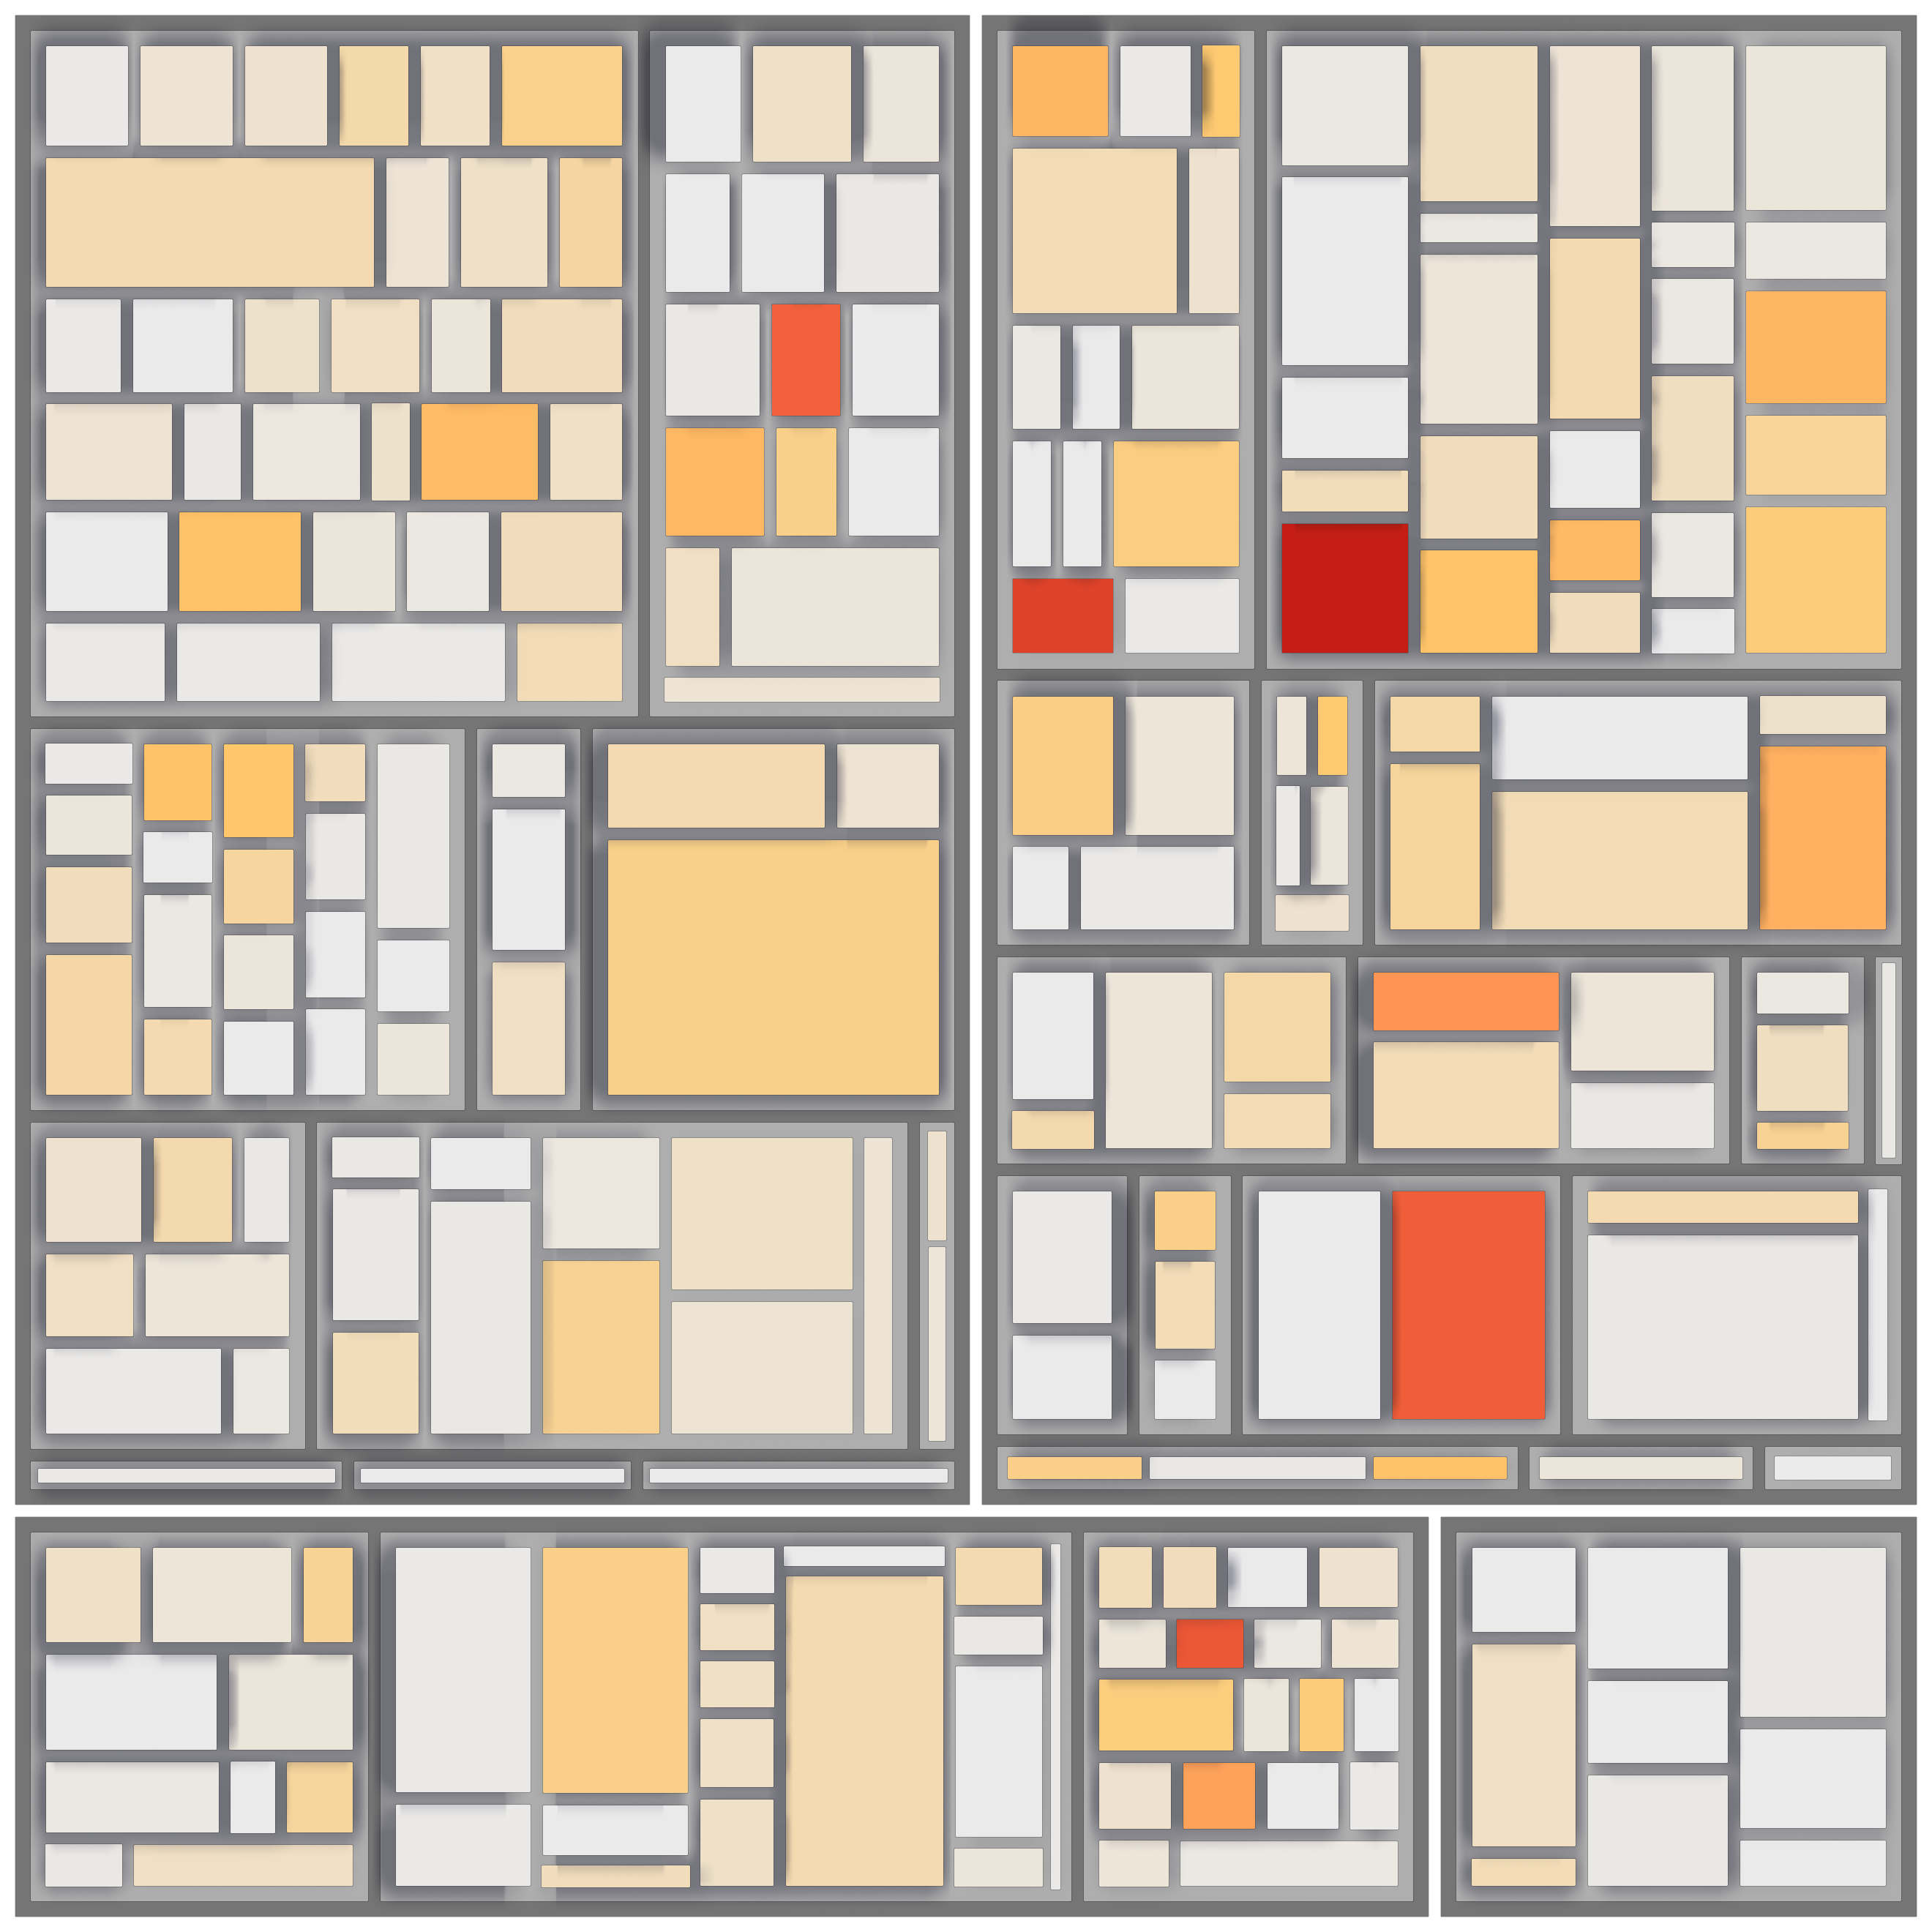
\includegraphics[width=0.9\linewidth]{images/tierpark-color.png}
		\end{column}
	\end{columns}
\end{frame}

\begin{frame}{Packing Layouts}
	\begin{columns}[T,onlytextwidth]
		\begin{column}{0.5\textwidth}
			\textbf{Packing Treemap Layouts}\par
			\smallskip
			\begin{itemize}
				\setlength{\itemsep}{10pt}
				\item Derivation of parent layout from child layouts \cite{schulz2011-implicit}
				\item Abstract layout algorithm for packing layouts
				\begin{enumerate}
					\item Assign root as current node
					\item Repeat 2--4 for all children nodes as current node
					\item If current node is leaf node, assign layout
					\item If current node is inner node, determine layout by placement of all child layouts and derivation of bounding box as own layout
				\end{enumerate}
				\item $\Rightarrow$ a bottom-up approach, iterating from leaf nodes to root node
			\end{itemize}
		\end{column}
		\begin{column}{0.5\textwidth}
			\centering
			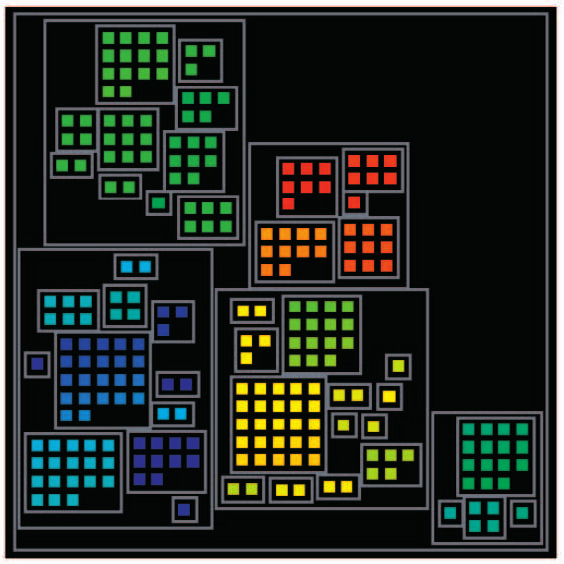
\includegraphics[width=0.9\linewidth]{images/data-jewelry-box.png}
		\end{column}
	\end{columns}
\end{frame}
